\documentclass[11pt,a4paper]{article}
\usepackage[utf8]{inputenc}
\usepackage[T1]{fontenc}
\usepackage[spanish,es-tabla]{babel}
\usepackage{lmodern,microtype,geometry,graphicx,booktabs,array,longtable,float}
\usepackage{amsmath,amssymb,xcolor,tikz,fancyhdr,titlesec,listings,hyperref}
\usetikzlibrary{arrows.meta,positioning,fit}
\geometry{left=24mm,right=24mm,top=25mm,bottom=25mm}
\definecolor{atlas}{HTML}{6554B8}
\definecolor{ink}{HTML}{292C36}
\definecolor{soft}{HTML}{F0EDF8}
\hypersetup{colorlinks=true,linkcolor=atlas,urlcolor=atlas,pdftitle={Atlas: motor multimodal y recomendador de productos},pdfauthor={Equipo CS2042}}
\setlength{\parindent}{0pt}
\setlength{\parskip}{6pt}
\setlength{\headheight}{14pt}
\renewcommand{\arraystretch}{1.2}
\pagestyle{fancy}\fancyhf{}
\fancyhead[L]{\small\textcolor{atlas}{ATLAS / BASE DE DATOS II}}
\fancyhead[R]{\small Entregable 2}
\fancyfoot[L]{\footnotesize CS2042 / 2026-II}
\fancyfoot[R]{\thepage}
\titleformat{\section}{\Large\bfseries\color{ink}}{\textcolor{atlas}{\thesection}}{.7em}{}
\titleformat{\subsection}{\large\bfseries\color{ink}}{\thesubsection}{.7em}{}
\lstset{basicstyle=\ttfamily\footnotesize,backgroundcolor=\color{soft},frame=none,breaklines=true,columns=fullflexible,keepspaces=true,xleftmargin=8pt,xrightmargin=8pt,aboveskip=12pt,belowskip=12pt}
\newcommand{\code}[1]{\texttt{#1}}
\begin{document}
\hypersetup{pageanchor=false}
\begin{titlepage}
\vspace*{12mm}
{\color{atlas}\Large\bfseries ATLAS\par}
\vspace{17mm}
{\fontsize{32}{38}\selectfont\bfseries Motor de bases de datos\\multimodal\par}
\vspace{7mm}
{\Large Recomendador visual de productos\\e índices persistentes en disco\par}
\vspace{13mm}
\colorbox{soft}{\parbox{.91\textwidth}{\vspace{5mm}\hspace{4mm}\textcolor{atlas}{\textbf{ENTREGABLE 2 / PROYECTO DEL CURSO}}\\[3mm]\hspace{4mm}R-Tree / Índice invertido / SIFT/BoVW / ResNet-18/IVF\vspace{5mm}}}
\vfill
{\large\textbf{Integrantes}\par}
Ivan Alonso Rodriguez Perez\\
Yacira Nicol Campoverde San Martín\\
Jorge Armando Martinez Palomino\\
Leonardo Alberto Montesinos Damian\par
\vspace{9mm}
\begin{tabular}{@{}ll}
Curso & Base de Datos II (CS2042)\\
Docente & Percy Lovon Ramos\\
Periodo & 2026-II\\
Fecha & 30 de octubre de 2026
\end{tabular}\par
\vspace{7mm}
{\small\url{https://github.com/Ivan-Alonso-Rodriguez/BD2_proyecto_Parte_2}\par}
\end{titlepage}
\hypersetup{pageanchor=true}
\tableofcontents
\newpage
\section{Resumen y alcance}
Atlas amplía el motor relacional del entregable 1 con recuperación espacial, textual y visual. El sistema implementa sus estructuras físicas mediante \code{struct}, \code{seek}, lecturas y escrituras de páginas de 4096 bytes. La API y el frontend consultan esos mismos archivos. No utiliza SQLite, PostgreSQL, FAISS ni otros motores para almacenar o consultar los datos de la aplicación.

La aplicación elegida es un recomendador de productos. Se cargaron 10000 imágenes y sus atributos reales de Fashion Product Images; se reservaron otras 100 imágenes, excluidas de los índices, para la evaluación visual. Los precios y las coordenadas de tienda se generan con semilla fija en torno a Lima y se identifican como sintéticos. Las descripciones concatenan atributos originales, con etiquetas de categoría en español.

La base heredada es \href{https://github.com/ArmandoPal/BD2_proyecto}{ArmandoPal/BD2\_proyecto}, en el commit \code{1634a747}. Se conserva su historial y se reutilizan Heap, RID, B+, Hash, DiskManager y el parser relacional. P2 añade módulos propios bajo \path{backend/core/multimodal} y preserva el cliente original en \path{frontend/sql.html}.

En las 100 consultas visuales separadas, la Precision@10 media fue 0.688 con ResNet-18/IVF y 0.295 con BoVW. Con cinco probes, IVF alcanzó Recall@10 de 97.1\%, con 34.09 ms y 690.03 lecturas medias por consulta. Estos resultados se derivan de los CSV versionados, no de valores teóricos.


\section{Arquitectura e integración}
\begin{figure}[H]\centering
\begin{tikzpicture}[node distance=8mm and 5mm,box/.style={draw=atlas!35,fill=soft,rounded corners=3pt,align=center,font=\small,minimum height=10mm},arr/.style={-{Stealth},draw=atlas!65}]
\node[box,minimum width=125mm] (ui) {Frontend: catálogo, imágenes, mapa Leaflet, SQL y experimentos};
\node[box,below=of ui,minimum width=125mm] (api) {FastAPI + parser SQL + planificador híbrido};
\node[box,below=of api,minimum width=29mm,xshift=-48mm] (b) {B+ / Hash\\Precio y categoría};
\node[box,right=of b,minimum width=27mm] (r) {R-Tree\\Geometrías};
\node[box,right=of r,minimum width=27mm] (t) {Invertido\\Texto y BoVW};
\node[box,right=of t,minimum width=27mm] (v) {IVF Flat\\ResNet-18};
\node[box,below=18mm of api,minimum width=125mm,yshift=-16mm] (heap) {RID $\langle page,slot\rangle$ $\rightarrow$ Heap de productos + cadenas de blobs};
\node[box,below=of heap,minimum width=125mm] (disk) {DiskManager / páginas de 4 KB / DiskCounter por tipo de archivo};
\draw[arr] (ui)--(api);\foreach \x in {b,r,t,v}{\draw[arr] (api)--(\x);\draw[arr] (\x)--(heap);}\draw[arr] (heap)--(disk);
\end{tikzpicture}
\caption{Flujo de la aplicación. PostgreSQL pertenece solo al entorno aislado del experimento 6.}
\end{figure}

\textbf{Integración física.} Cada fila ocupa 780 bytes y mantiene el RID del Heap de P1. Los índices P2 empaquetan ese RID como entero de 64 bits: $page\_id\cdot 2^{32}+slot$. El identificador comercial de la imagen permanece en la columna \code{id}. El catálogo JSON contiene esquemas y rutas; nunca filas ni listas de posteo.

\textbf{Instrumentación.} DiskCounter aumenta únicamente al completar una transferencia de página en DiskManager. Distingue tabla, índice y blob. Las cabeceras también cuentan. Los archivos están abiertos sin buffering de Python; la caché del sistema operativo no se vacía. Por ello, las lecturas registradas no equivalen a accesos físicos al dispositivo ni a fallos de caché del SO. La recuperación por RID y los arreglos usan cachés locales acotadas, nuevas en cada consulta.

\textbf{Preprocesamiento offline.} Los cachés NumPy de SIFT y ResNet se usan durante construcción y evaluación; no son índices y la API no los lee al resolver búsquedas. Los pesos de ResNet son un modelo preentrenado externo, no un mecanismo de almacenamiento del motor.

\section{Diseño físico de los índices}
\subsection{R-Tree y recuperación geográfica}
La página cero guarda magic, versión, dimensión, raíz, capacidad y cantidad. Cada nodo inicia con \code{<4sIBH>} (11 bytes); una entrada 2D ocupa 40 bytes: cuatro coordenadas float64 y una referencia de 64 bits. Caben 102 entradas por página. En hojas la referencia es un RID; en internos apunta a una página hija.

\begin{figure}[H]\centering
\begin{tikzpicture}[font=\small]
\draw[fill=soft,draw=atlas!50] (0,0) rectangle (14,1.3);
\draw (2.8,0)--(2.8,1.3);\draw (6.7,0)--(6.7,1.3);\draw (10.6,0)--(10.6,1.3);
\node[align=center] at (1.4,.65) {Cabecera\\11 bytes};
\node[align=center] at (4.75,.65) {MBR + ref\\40 bytes};
\node[align=center] at (8.65,.65) {MBR + ref\\40 bytes};
\node[align=center] at (12.3,.65) {$\cdots$ hasta 102\\entradas};
\end{tikzpicture}
\caption{Nodo R-Tree 2D en una página física de 4096 bytes.}
\end{figure}

La inserción desciende por mínima ampliación de área; los empates usan el área actual. El split lineal elige semillas por máxima separación normalizada de extremos y reparte entradas respetando ocupación mínima de 40\%. Los MBR y splits se propagan hacia la raíz, cuya dirección se persiste. Las consultas por ventana podan cajas disjuntas. k-NN usa una cola mínima de páginas por MINDIST y un max-heap de los mejores resultados.

La aplicación transforma un radio en km en una o dos ventanas lon/lat, cubriendo antimeridiano y polos, y refina con Haversine. El k-NN geográfico utiliza una cota esférica admisible al MBR. En el experimento de dimensionalidad, D$>$2 usa float32 redondeado hacia afuera; esa reducción permite al menos tres entradas aun en D=128.

\subsection{Diccionario, posteos y normas}
El pipeline normaliza Unicode, convierte a minúsculas, elimina stopwords ES/EN y aplica Snowball. El catálogo usa stemming inglés porque sus títulos y atributos provienen de un corpus en inglés; el analizador español también está implementado y probado.

\begin{table}[H]\centering\small
\begin{tabular}{@{}lll@{}}\toprule
Archivo & Registro binario & Acceso\\\midrule
\code{vocab.dic} & \code{<128sQQQ>}: término, df, offset, longitud & Binaria por término\\
\code{postings.inv} & \code{<QI>}: doc\_id, tf & Lista por offset\\
\code{norms.norm} & \code{<Qd>}: doc\_id, norma & Binaria por doc\_id\\\bottomrule
\end{tabular}\caption{Archivos del índice invertido; todos se organizan en páginas de 4 KB.}
\end{table}

Los registros de los arreglos no cruzan límites de página. El diccionario ordenado permite localizar solo los términos consultados sin reconstruirlo entero en RAM. Sus offsets son direcciones físicas en posteos. Cada lista está ordenada por doc\_id. AND, OR y AND-NOT usan mezcla con dos punteros, de complejidad $O(n+m)$.

\[
w_{t,d}=(1+\log_{10}tf_{t,d})\log_{10}\frac{N}{df_t},\qquad
score(q,d)=\frac{\sum_{t\in q} w_{t,q}w_{t,d}}{\lVert q\rVert_2\lVert d\rVert_2}.
\]
Las normas de documento se calculan al construir y se persisten. El ranking acumula productos únicamente sobre los posteos de consulta y selecciona Top-K con heap. Los vectores de norma cero no generan divisiones inválidas; una coincidencia booleana de score cero sigue siendo válida.

\subsection{BoVW y embeddings profundos}
OpenCV extrae SIFT 128D sobre imágenes redimensionadas a $224\times224$, con hasta 100 puntos por imagen. Un K-Means de Lloyd implementado con NumPy entrena 128 palabras visuales sobre hasta 30000 descriptores muestreados del corpus indexado, sin usar consultas. Cada imagen se convierte en frecuencias de palabras visuales y se indexa con el mismo mecanismo TF-IDF/coseno.

El paradigma denso emplea ResNet-18 con pesos ImageNet \code{IMAGENET1K\_V1}. Se reemplaza la capa final por identidad; la salida de 512D se normaliza en L2. La extracción aplica el preprocesamiento oficial de Torchvision. No se entrenó la red con etiquetas del experimento y no se fabricaron embeddings.

\subsection{IVF Flat paginado y búsqueda exacta}
Se entrenan $C=\lfloor\sqrt{10000}\rfloor=100$ centroides mediante K-Means propio; para coseno se normalizan vectores y centroides. El directorio almacena cluster, vector centroide, página inicial y cantidad. Las listas enlazadas contienen RID y vector float32.

\begin{figure}[H]\centering
\begin{tikzpicture}[node distance=7mm and 7mm,box/.style={draw=atlas!40,fill=soft,rounded corners,minimum height=10mm,align=center,font=\small},arr/.style={-{Stealth},draw=atlas!70}]
\node[box,minimum width=40mm] (c) {Centroide $\mu_c$\\head\_page, cantidad};
\node[box,right=of c,minimum width=30mm] (p1) {Página $p$\\RID + vector};
\node[box,right=of p1,minimum width=30mm] (p2) {Página $p+1$\\RID + vector};
\node[right=of p2] (end) {$\cdots\rightarrow -1$};
\draw[arr] (c)--(p1);\draw[arr] (p1)--(p2);\draw[arr] (p2)--(end);
\end{tikzpicture}
\caption{Directorio de centroides y listas paginadas IVF. Solo se recorren las listas elegidas.}
\end{figure}

Cada vector de 512D más RID ocupa 2056 bytes. Con cabecera de 16 bytes cabe una entrada por página; se privilegia simplicidad y trazabilidad a costa de ocupación cercana al 50\%. El benchmark refleja ese costo, sin simular empaquetamiento más eficiente.

La consulta lee el directorio de centroides, escoge los probes más cercanos y mantiene un max-heap Top-K al recorrer sus listas. El archivo \code{vectors.vec}, ordenado por RID, conserva la línea base exacta. Con todos los centroides, IVF coincide con el escaneo exacto; esa equivalencia se verifica en tests y en el catálogo real. Se soportan coseno, L2 y un filtro de distancia máxima en la línea base.

\newpage
\section{SQL, planificación híbrida y aplicación}
\begin{lstlisting}
SELECT id, titulo, precio, COSINE_SCORE() AS relevancia
FROM productos
WHERE cuerpo MATCH 'black AND shoes AND NOT women'
AND precio <= 250 AND categoria = 'Footwear'
ORDER BY relevancia DESC LIMIT 10;

SELECT id, titulo, ubicacion FROM productos
WHERE ubicacion WITHIN_RADIUS ((-77.04, -12.10), 2.5)
LIMIT 20;

SET ivf.probes = 5;
CREATE INDEX visual_v2 ON productos(embedding)
USING IVF WITH (lists=100, metric='COSINE');
\end{lstlisting}

La extensión admite \code{MATCH}, \code{WITHIN\_RADIUS}, \code{COSINE\_SCORE()}, \code{<=>}, \code{<->}, ORDER BY, LIMIT y CREATE INDEX de los tres tipos. El vector SQL es un literal JSON con las 512 dimensiones completas. La API también permite una imagen o el ID de un producto como referencia.

El planificador aplica B+ de precio o Hash de categoría, intersecta RID, verifica filtros estrictos, aplica el filtro espacial/textual y recupera similitud. Es un planificador por reglas, no un optimizador estadístico. En IVF, descartar RID por filtros reduce evaluaciones y resultados, pero no evita leer las páginas correspondientes dentro de una lista elegida.

El frontend permite subir una foto, buscar por descripción, comparar BoVW/IVF/exacto, cambiar probes, filtrar por precio/categoría y mover el centro del radio sobre un mapa. La consola ejecuta SQL real. Los resultados muestran latencia, lecturas, escrituras, desglose por archivo y los pasos ejecutados. Los errores limpian métricas y resultados anteriores.

\IfFileExists{../docs/images/catalog.png}{\begin{figure}[H]\centering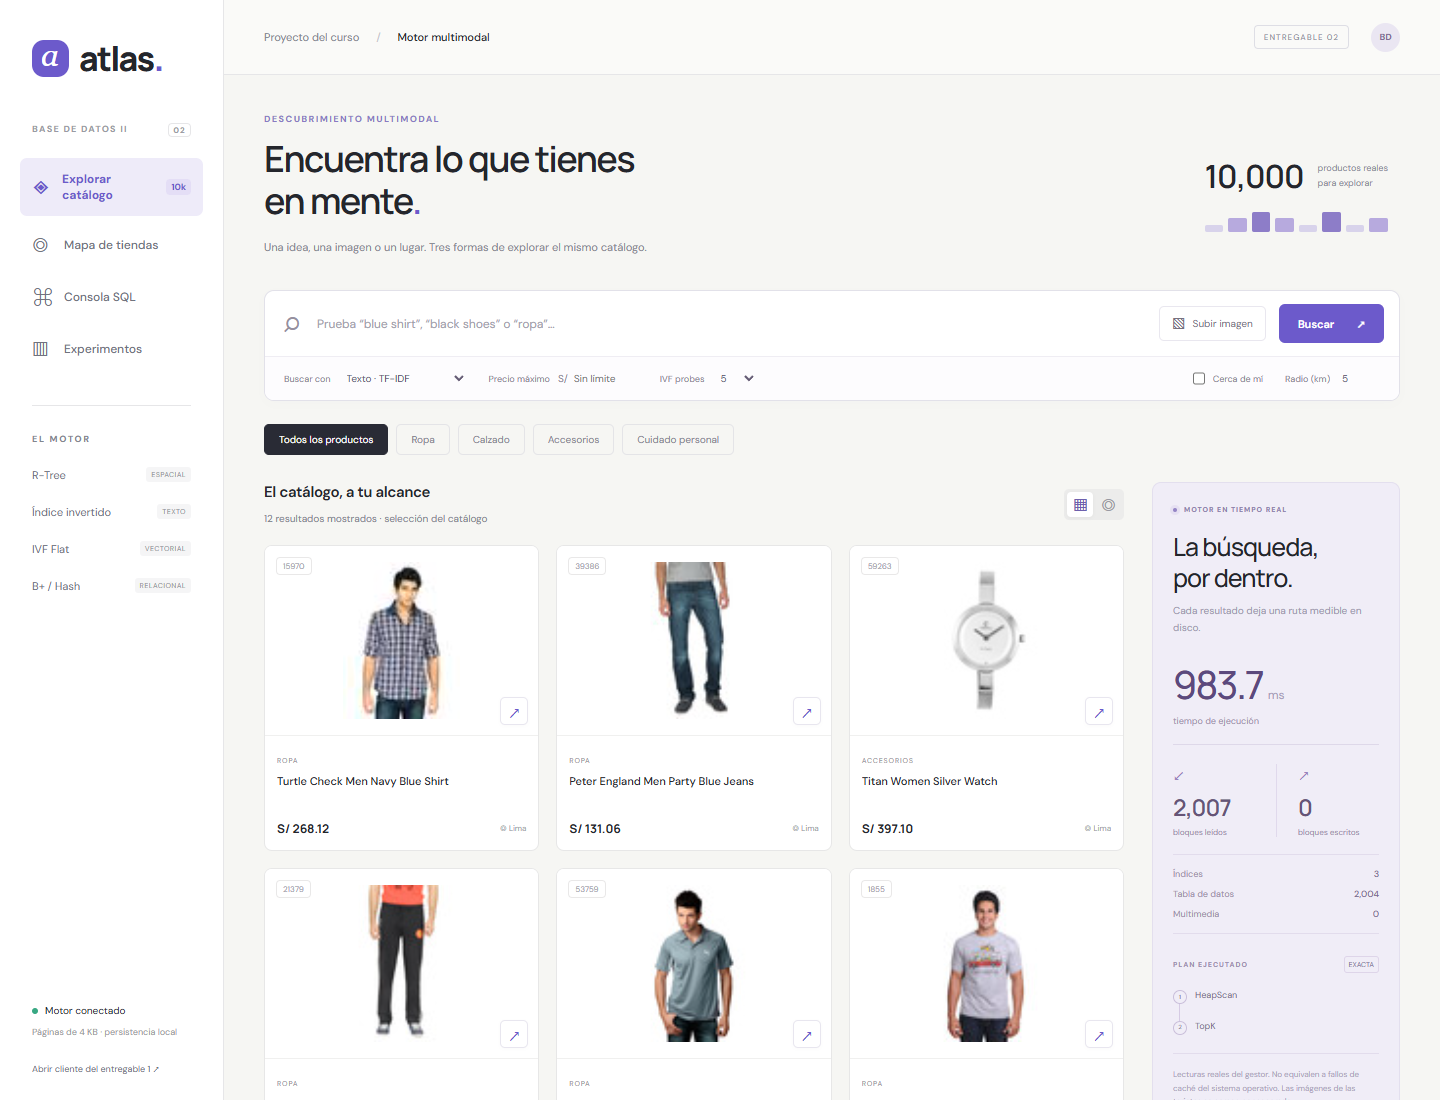
\includegraphics[width=.85\textwidth,height=.37\textheight,keepaspectratio]{../docs/images/catalog.png}\caption{Interfaz ejecutada sobre el catálogo real. Captura de validación del navegador.}\end{figure}}{}

\newpage
\section{Metodología experimental}
Los experimentos generan CSV crudos, resúmenes con media y desviación estándar poblacional, gráficas y metadata del entorno. Se usan semillas fijas. Las consultas abren objetos de índice nuevos; no se vacía la caché del sistema operativo. El tiempo incluye apertura y lectura de metadata. Las cifras no son garantías de rendimiento en otros equipos.

\begin{table}[H]\centering\small
\begin{tabular}{@{}lp{10.5cm}@{}}\toprule
Experimento & Diseño\\\midrule
5 & N=10000, 50000, 100000; k=5,20,50; radios 0.005,0.02,0.05 grados; 12 centros por configuración. Dimensiones 2,4,8,16,32,64,128 con N=2000 y k=10.\\
6 & Corpus real de 1000,5000,10000,20000 documentos; AND, OR, AND-NOT y ranking; 1,3,5 términos; tres consultas distintas por combinación.\\
7 & 100 imágenes de consulta no indexadas; relevancia por coincidencia exacta de articleType. Precision@5 y @10; extracción y consulta por separado.\\
8 & Mismas 100 consultas; ground truth k-NN exacto coseno; probes=1,2,5,10,20,50,100; Recall@10, ms e I/O.\\\bottomrule
\end{tabular}\caption{Diseño de los cuatro experimentos del entregable 2.}
\end{table}

\textbf{Precauciones de interpretación.} En el experimento 5 los radios en grados son planarios, para comparar estructuras con idéntica métrica; la aplicación usa kilómetros y Haversine. El experimento de dimensión mantiene N=2000 y cambia tanto D como la capacidad del nodo. Por ello, el resultado combina solapamiento y fan-out, y no constituye un umbral universal de dimensionalidad.

El Full Scan textual lee texto normalizado materializado y norma L2; no recorre posteos. Sus IDF provienen de estadísticas construidas offline. PostgreSQL usa los mismos tokens Snowball con configuración \code{simple}; se desactiva SeqScan para aislar el acceso GIN. La construcción propia incluye análisis léxico, mientras PostgreSQL recibe tokens ya normalizados: ese costo no es estrictamente equivalente. GIN se mide por índice; el tamaño propio incluye vocabulario y posteos, excluyendo normas.

El ranking PostgreSQL usa \code{ts\_rank\_cd}, no la fórmula TF-IDF del motor; la comparación de latencia no implica igualdad de relevancia. Las consultas booleanas sí verifican igualdad de conjuntos entre los tres métodos. El tiempo PostgreSQL incluye ida/vuelta al contenedor local; sus shared hit/read de 8 KB se almacenan aparte de las lecturas de 4 KB de Atlas. Los planes EXPLAIN completos quedan versionados.

\clearpage\section{Resultados y análisis}

\subsection{Experimento 5: escalabilidad espacial}

\begin{table}[H]\centering\small
\caption{k-NN y radio planar de 0.02 grados; doce centros por tamaño.}
\begin{tabular}{@{}lrrrrr@{}}\toprule
N & Consulta & Método & Lecturas & Media ms & Desv. ms \\ \midrule
10000 & k=20 & Sequential & 60.00 & 9.74 & 1.95 \\
10000 & k=20 & RTree & 10.67 & 1.85 & 0.43 \\
10000 & r=0.02 & Sequential & 60.00 & 9.02 & 1.40 \\
10000 & r=0.02 & RTree & 97.17 & 4.00 & 1.16 \\
50000 & k=20 & Sequential & 296.00 & 40.20 & 2.34 \\
50000 & k=20 & RTree & 16.92 & 2.68 & 0.60 \\
50000 & r=0.02 & Sequential & 296.00 & 37.89 & 3.48 \\
50000 & r=0.02 & RTree & 631.92 & 12.85 & 1.48 \\
100000 & k=20 & Sequential & 590.00 & 108.20 & 9.69 \\
100000 & k=20 & RTree & 25.17 & 4.93 & 1.26 \\
100000 & r=0.02 & Sequential & 590.00 & 95.14 & 9.69 \\
100000 & r=0.02 & RTree & 1381.42 & 35.71 & 5.47 \\
\bottomrule\end{tabular}\end{table}

\begin{figure}[H]\centering
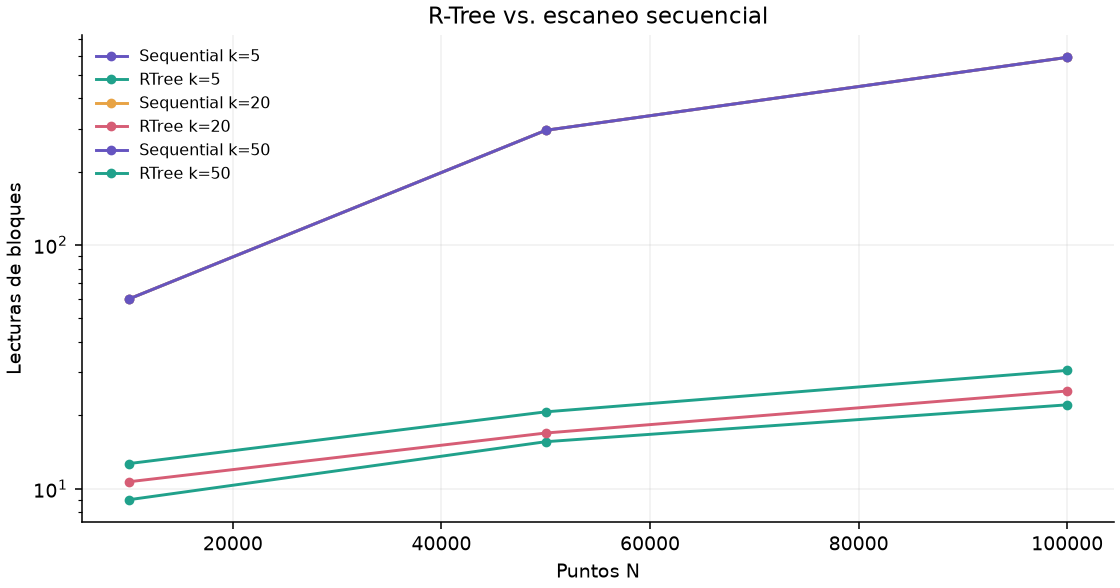
\includegraphics[width=.89\textwidth]{../benchmarks/p2/results/exp5_spatial.png}
\caption{Escalabilidad k-NN para k=5,20,50. Eje de I/O logarítmico.}\end{figure}

Con 100000 puntos y k=20, el R-Tree leyó 25.17 bloques en promedio frente a 590.00 del escaneo. La poda evita recorrer la mayoría de las páginas en este conjunto 2D. La comparación k-NN devuelve identificadores: no incluye recuperar filas comerciales del Heap. En radios sí se contabiliza el refinamiento desde el archivo de puntos. Los CSV crudos incluyen los tres radios y todos los k.

En radio r=0.02 y N=100000, el R-Tree con refinamiento lee 1381.42 bloques, más que el escaneo. Los candidatos espaciales están dispersos en el archivo y provocan relecturas con la caché acotada. Aun así, su latencia es menor al evaluar menos puntos. Un índice selectivo no garantiza por sí solo menor I/O al recuperar datos no agrupados.

\clearpage\subsection{Experimento 5: efecto de la dimensión}

\begin{table}[H]\centering\small
\caption{2000 vectores uniformes por dimensión, doce consultas k=10.}
\begin{tabular}{@{}lrrrr@{}}\toprule
D & Scan I/O & R-Tree I/O & Scan ms & R-Tree ms \\ \midrule
2 & 13.00 & 6.50 & 3.69 & 2.13 \\
4 & 21.00 & 8.83 & 3.09 & 2.77 \\
8 & 37.00 & 41.58 & 4.28 & 9.64 \\
16 & 68.00 & 98.00 & 5.66 & 23.31 \\
32 & 135.00 & 174.00 & 9.51 & 45.16 \\
64 & 287.00 & 385.00 & 16.41 & 96.50 \\
128 & 668.00 & 1104.00 & 30.34 & 238.83 \\
\bottomrule\end{tabular}\end{table}

\begin{figure}[H]\centering
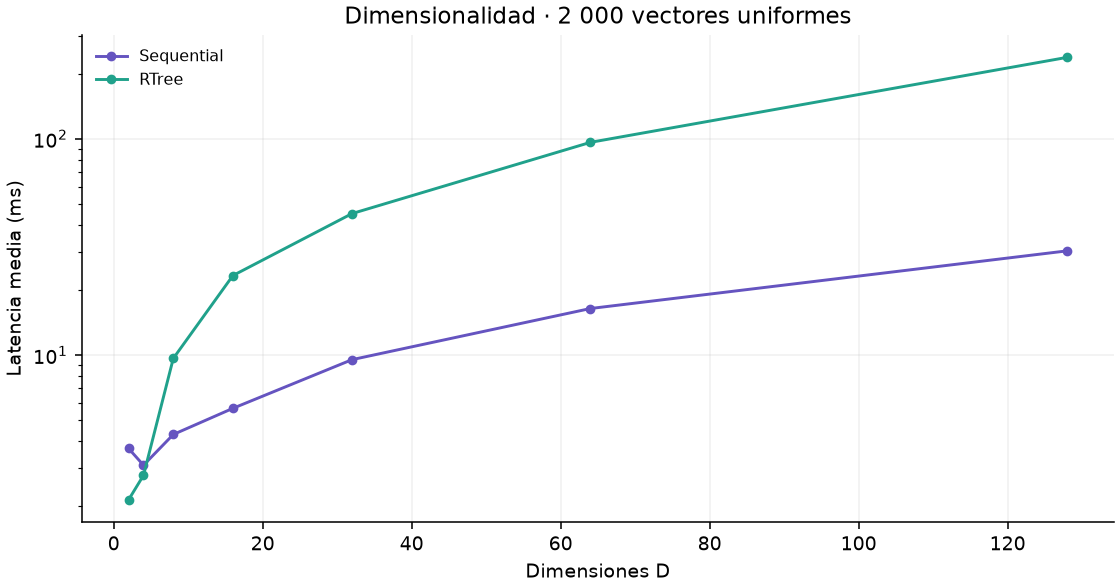
\includegraphics[width=.89\textwidth]{../benchmarks/p2/results/exp5_dimensions.png}
\caption{Costo temporal al aumentar D; escala logarítmica.}\end{figure}

El primer D medido donde la media del árbol supera al escaneo es 8. A dimensiones elevadas, la búsqueda visita una fracción creciente del árbol y disminuye el fan-out. Este cruce depende de la distribución, la implementación y el hardware; no debe generalizarse como una dimensión límite universal.

\clearpage\subsection{Experimento 6: construcción y espacio}

\begin{table}[H]\centering\small
\caption{Construcción y tamaño del diccionario/posteos propios frente al índice GIN.}
\begin{tabular}{@{}lrrr@{}}\toprule
N & Método & Construcción ms & Índice KiB \\ \midrule
1000 & Inverted & 194.62 & 304.0 \\
1000 & PostgreSQL GIN & 228.02 & 104.0 \\
5000 & Inverted & 853.07 & 1072.0 \\
5000 & PostgreSQL GIN & 123.42 & 304.0 \\
10000 & Inverted & 1699.46 & 1964.0 \\
10000 & PostgreSQL GIN & 156.66 & 536.0 \\
20000 & Inverted & 3340.37 & 3624.0 \\
20000 & PostgreSQL GIN & 273.10 & 960.0 \\
\bottomrule\end{tabular}\end{table}

\begin{figure}[H]\centering
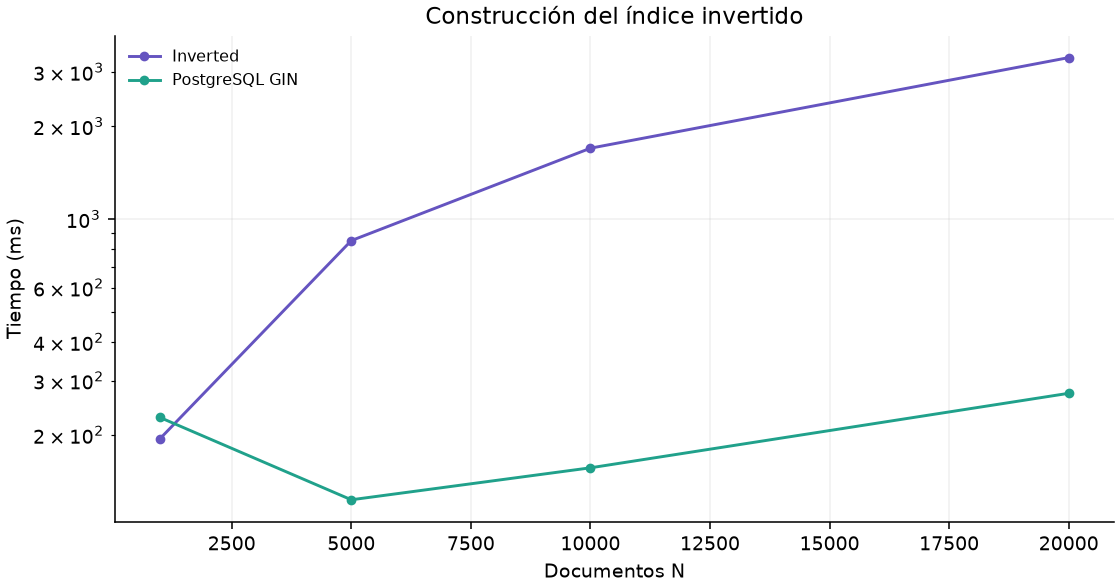
\includegraphics[width=.48\textwidth]{../benchmarks/p2/results/exp6_build.png}
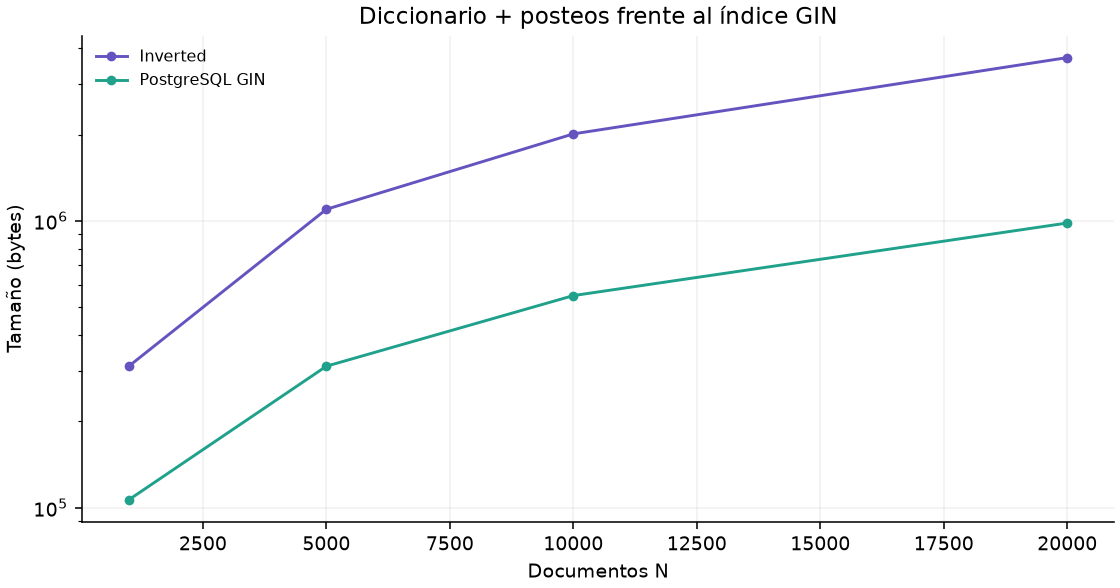
\includegraphics[width=.48\textwidth]{../benchmarks/p2/results/exp6_size.png}
\caption{Crecimiento temporal y espacial. Los archivos de normas se excluyen del tamaño propio solicitado.}\end{figure}

El índice propio usa registros de diccionario de tamaño fijo y posteos sin compresión; GIN utiliza una representación distinta y comprime identificadores. Los costos de construcción también incluyen trabajo diferente de normalización y de base de datos, por lo que la tabla describe implementaciones completas bajo las condiciones documentadas, no una comparación aislada de un algoritmo idéntico.

\clearpage\subsection{Experimento 6: consultas y transferencias}

\begin{table}[H]\centering\footnotesize\renewcommand{\arraystretch}{1.0}
\caption{Latencias medias sobre 20000 documentos; tres consultas distintas por combinación.}
\begin{tabular}{@{}lrrrr@{}}\toprule
Términos & Consulta & Full Scan ms & Invertido ms & GIN ms \\ \midrule
1 & AND & 325.70 & 4.94 & 2.91 \\
1 & OR & 321.58 & 5.36 & 2.74 \\
1 & AND-NOT & 325.85 & 5.09 & 2.76 \\
1 & RANK & 349.69 & 35.44 & 56.66 \\
3 & AND & 321.56 & 18.98 & 2.15 \\
3 & OR & 325.34 & 21.08 & 6.37 \\
3 & AND-NOT & 320.30 & 20.98 & 2.61 \\
3 & RANK & 369.49 & 134.17 & 601.88 \\
5 & AND & 322.86 & 21.09 & 1.49 \\
5 & OR & 330.72 & 29.05 & 6.99 \\
5 & AND-NOT & 316.44 & 28.49 & 2.71 \\
5 & RANK & 372.73 & 146.09 & 1068.13 \\
\bottomrule\end{tabular}\end{table}

\begin{table}[H]\centering\footnotesize\renewcommand{\arraystretch}{1.0}
\caption{Transferencias Atlas y buffers PostgreSQL reportados por separado.}
\begin{tabular}{@{}lrrrrr@{}}\toprule
Términos & Consulta & Scan 4K & Inv. 4K & PG hit 8K & PG read 8K \\ \midrule
1 & AND & 6668.0 & 23.0 & 784.0 & 0.0 \\
1 & OR & 6668.0 & 23.0 & 784.0 & 0.0 \\
1 & AND-NOT & 6668.0 & 23.0 & 784.0 & 0.0 \\
1 & RANK & 6668.0 & 102.0 & 784.0 & 0.0 \\
3 & AND & 6668.0 & 84.0 & 392.0 & 0.0 \\
3 & OR & 6668.0 & 84.0 & 802.0 & 0.0 \\
3 & AND-NOT & 6668.0 & 84.0 & 550.3 & 0.0 \\
3 & RANK & 6668.0 & 319.0 & 802.0 & 0.0 \\
5 & AND & 6668.0 & 103.7 & 19.3 & 0.0 \\
5 & OR & 6668.0 & 103.7 & 806.7 & 0.0 \\
5 & AND-NOT & 6668.0 & 103.7 & 540.7 & 0.0 \\
5 & RANK & 6668.0 & 471.0 & 806.7 & 0.0 \\
\bottomrule\end{tabular}\end{table}

OR y ranking consultan conjuntos mayores cuando los términos son frecuentes. AND puede reducir resultados por intersección. Los planes PostgreSQL completos permiten distinguir navegación GIN, acceso a Heap y ordenamiento. El ranking ts\_rank\_cd tiene costo y semántica diferentes de TF-IDF/coseno; una menor latencia de Atlas en un caso no demuestra superioridad general frente a PostgreSQL.

\begin{figure}[H]\centering
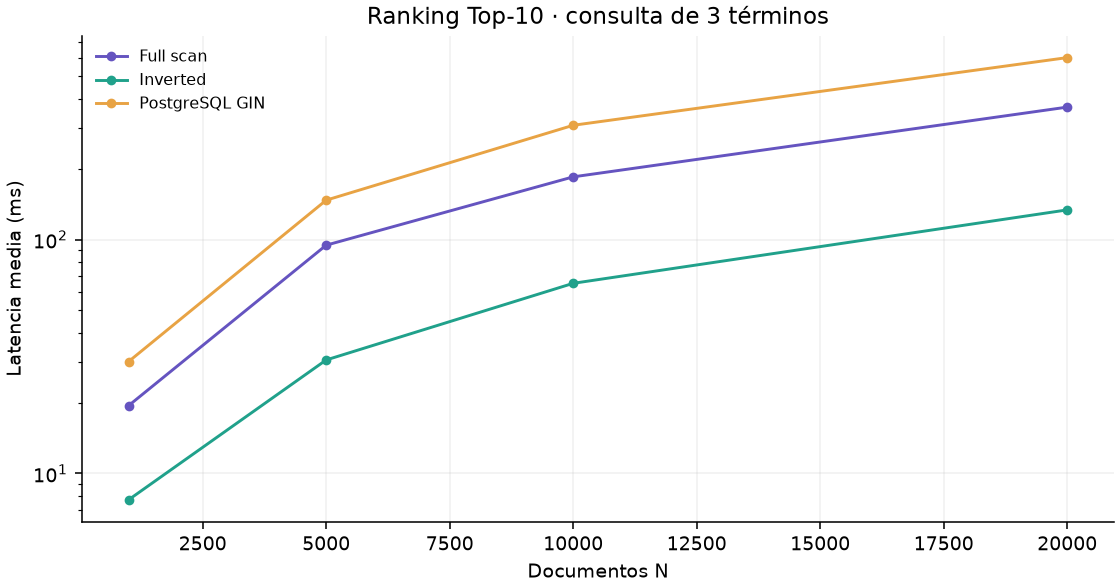
\includegraphics[width=.66\textwidth]{../benchmarks/p2/results/exp6_query.png}
\caption{Ranking Top-10 de tres términos según tamaño del corpus.}\end{figure}

\clearpage\subsection{Experimento 7: BoVW frente a embeddings}

\begin{table}[H]\centering\small
\caption{100 imágenes de consulta excluidas del corpus indexado.}
\begin{tabular}{@{}lrrrr@{}}\toprule
Método & P@5 & P@10 & Consulta ms & Extracción ms/img \\ \midrule
BoVW & 0.330 & 0.295 & 164.35 & 7.07 \\
ResNet18+IVF & 0.702 & 0.688 & 35.00 & 26.16 \\
\bottomrule\end{tabular}\end{table}

\begin{figure}[H]\centering
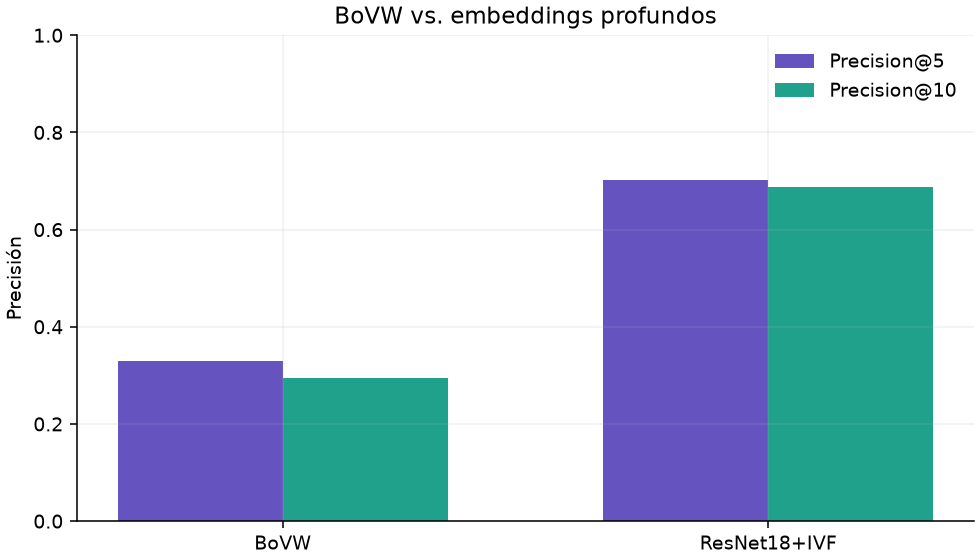
\includegraphics[width=.89\textwidth]{../benchmarks/p2/results/exp7_quality.png}
\caption{Relevancia definida por igualdad de articleType.}\end{figure}

ResNet-18 obtuvo mayor precisión por categoría en este conjunto. BoVW reconoce patrones locales que pueden repetirse entre objetos de categorías distintas, mientras las características profundas incorporan representaciones aprendidas en ImageNet. La extracción densa es más costosa por imagen en la CPU usada. La consulta BoVW incluye cuantización contra el codebook; su carga inicial se reutiliza en este benchmark. Los tiempos de extracción son medias de lotes de preparación, no latencias individuales de una imagen interactiva.

\clearpage\subsection{Experimento 8: recall, latencia e I/O}

\begin{table}[H]\centering\small
\caption{Compromiso de IVF contra la búsqueda exacta sobre las mismas 100 consultas.}
\begin{tabular}{@{}lrrrr@{}}\toprule
Probes & Recall@10 & Media ms & Desv. ms & Lecturas medias \\ \midrule
1 & 67.2\% & 13.05 & 4.10 & 228.63 \\
2 & 86.2\% & 18.64 & 6.08 & 351.33 \\
5 & 97.1\% & 34.09 & 11.39 & 690.03 \\
10 & 99.2\% & 60.63 & 18.65 & 1251.39 \\
20 & 99.8\% & 112.63 & 32.20 & 2331.02 \\
50 & 100.0\% & 239.19 & 50.95 & 4962.69 \\
100 & 100.0\% & 477.61 & 75.26 & 10103.00 \\
\bottomrule\end{tabular}\end{table}

\begin{figure}[H]\centering
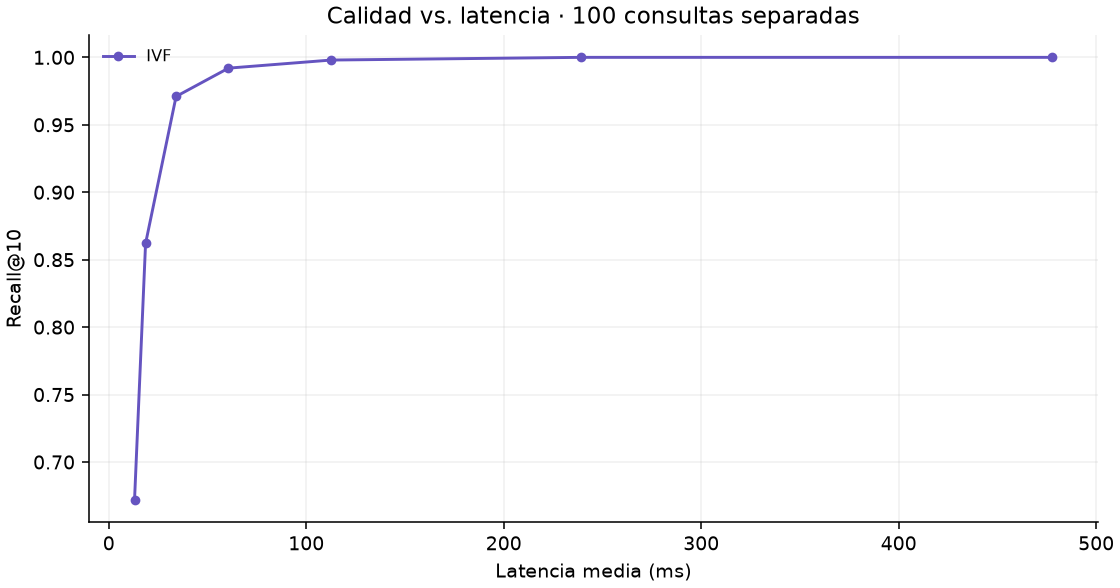
\includegraphics[width=.48\textwidth]{../benchmarks/p2/results/exp8_recall_latency.png}
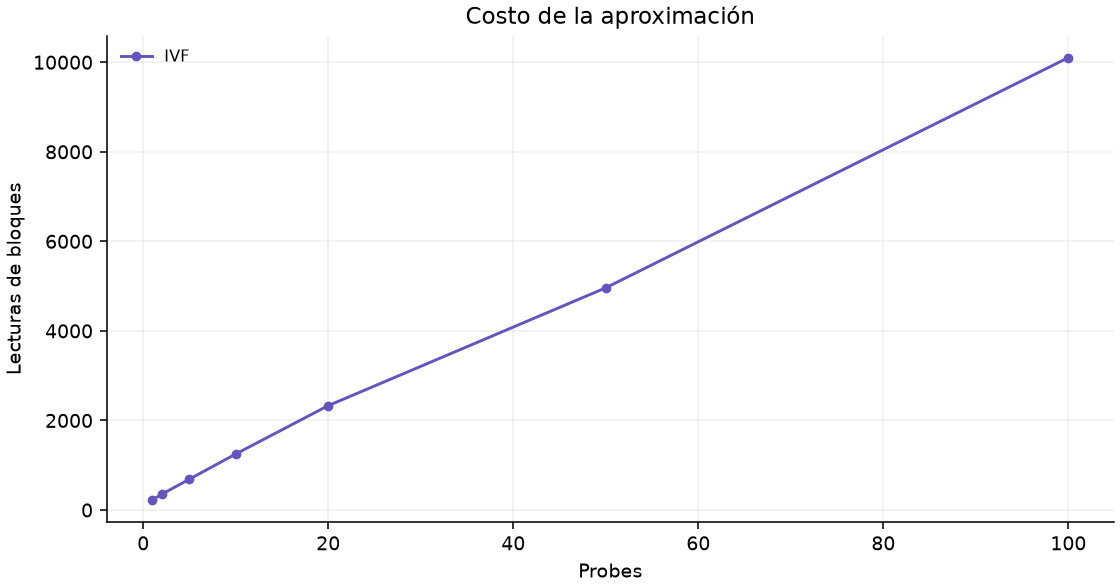
\includegraphics[width=.48\textwidth]{../benchmarks/p2/results/exp8_reads.png}
\caption{La exploración de más listas aumenta calidad y costo de consulta.}\end{figure}

Cinco probes ofrecen un punto de operación favorable en estas mediciones: 97.1\% de recall medio, sin explorar todo el índice. Los cien probes recorren todas las listas y garantizan la equivalencia con el escaneo exacto. Un recall de 100\% observado con menos probes solo aplica a las consultas medidas. La latencia incluye directorio y apertura; el conteo incluye metadata y listas, no recuperación de la ficha comercial.


\clearpage
\section{Reproducibilidad, validación y despliegue}
La última suite registrada ejecutó 114 pruebas, con 0 fallos o errores. Se verificaron 10000 registros y 100 imágenes tras reabrir los archivos. El entorno registrado utiliza Python 3.12.14 sobre Windows-11-10.0.26200-SP0. Las versiones exactas se guardan en requirements-lock.txt y environment.json.

La verificación del catálogo reabre los archivos, compara los 10000 RID del Heap con R-Tree, normas e IVF, comprueba 100 JPEG y verifica la igualdad de IVF con todos los probes y búsqueda exacta. La suite cubre splits, duplicados, persistencia, fórmulas, consultas híbridas, entradas inválidas y regresiones P1. El navegador se verificó en escritorio y a 390 píxeles de ancho, con captura de catálogo, mapa, búsqueda visual y SQL.

\begin{lstlisting}
# Preparar todo e iniciar API + frontend
python setup.py --full
# Inicios posteriores, entorno virtual activo
python run.py
# Pruebas
python -m pytest backend/tests -q
python tools/validate_multimodal.py
# PostgreSQL solo para benchmark
docker compose --profile benchmark up -d postgres
python -m benchmarks.p2.run_all
# Informe (Tectonic o pdflatex en PATH)
python tools/build_p2_report.py
\end{lstlisting}

La aplicación se sirve en \url{http://127.0.0.1:8000}; FastAPI publica la documentación en /docs. También se incluye Dockerfile y Compose con volumen persistente para datos y pesos. El despliegue validado es local; no se afirma un alojamiento público de la aplicación. El repositorio contiene código, resultados, informe y guion de sustentación, sin incluir el dataset masivo ni pesos.

\section{Límites y mejoras}
La colección multimodal publicada es de solo lectura. Se bloquean INSERT, DELETE y DROP para impedir desincronizar los índices. P1 mantiene sus operaciones sobre las demás tablas. La reconstrucción se realiza en otro directorio y CREATE INDEX publica una nueva ruta al finalizar; se conservan los archivos anteriores.

No hay WAL, recuperación transaccional ni coordinación de escritores entre procesos. La construcción textual y el entrenamiento necesitan RAM proporcional al corpus; SPIMI sería la extensión para corpus mayores. IVF desperdicia espacio por el registro de 512D; páginas de 8 KB o empaquetamiento de vectores por fragmentos podrían mejorarlo. El diccionario binario y las normas ordenadas admiten optimizaciones de localidad sin cambiar la semántica.

La evaluación visual usa imágenes pequeñas y una etiqueta de categoría como proxy de relevancia. No mide preferencias de usuarios, calidad de prendas ni disponibilidad real. El desbalance de categorías puede influir en Precision@K. El sistema carece de autenticación y se ejecuta en localhost.

La grabación final de 5-10 minutos requiere participación real de los cuatro integrantes. Se entrega un guion con recorrido técnico y preguntas de sustentación; no se atribuye al equipo una grabación o exposición que no haya realizado.

\section{Conclusiones}
La persistencia de índices y la separación de accesos permiten explicar el costo de cada consulta desde sus páginas. R-Tree mejora consultas selectivas 2D y pierde eficiencia al aumentar la dimensión del experimento. El índice invertido evita explorar todo el corpus para consultas selectivas, aunque los términos frecuentes y las normas pueden elevar su costo. Las representaciones profundas mejoran la precisión por categoría observada frente al vocabulario SIFT, a cambio de mayor costo de extracción. IVF ofrece un parámetro explícito para intercambiar exhaustividad por latencia e I/O; los resultados medidos permiten elegir probes sin ocultar pérdida de recall.

\begin{thebibliography}{9}
\raggedright
\bibitem{guttman} A. Guttman. \emph{R-Trees: A Dynamic Index Structure for Spatial Searching}. ACM SIGMOD, 1984. \url{https://doi.org/10.1145/602259.602266}.
\bibitem{ir} C. Manning, P. Raghavan y H. Schütze. \emph{Introduction to Information Retrieval}. Cambridge University Press, 2008. \url{https://nlp.stanford.edu/IR-book/}.
\bibitem{sift} D. Lowe. \emph{Distinctive Image Features from Scale-Invariant Keypoints}. IJCV, 2004. \url{https://www.cs.ubc.ca/~lowe/papers/ijcv04.pdf}.
\bibitem{resnet} Torchvision. \emph{ResNet-18 y pesos ImageNet}. \url{https://docs.pytorch.org/vision/stable/models/generated/torchvision.models.resnet18.html}.
\bibitem{data} P. Aggarwal. \emph{Fashion Product Images (Small)}. Kaggle. Copia de distribución: \url{https://huggingface.co/datasets/ashraq/fashion-product-images-small}. Revisión y SHA-256 conservados en evidencia.
\bibitem{gin} PostgreSQL 17. \emph{Preferred Index Types for Text Search; Using EXPLAIN}. \url{https://www.postgresql.org/docs/17/textsearch-indexes.html}; \url{https://www.postgresql.org/docs/17/using-explain.html}.
\bibitem{leaflet} Leaflet 1.9.4. \emph{API Reference}. \url{https://leafletjs.com/reference.html}.
\end{thebibliography}
\end{document}
